\hypertarget{duxe9tente-uxe0-carthaguxe8ne-des-indes}{%
\section{Détente à
Carthagène-des-Indes}\label{duxe9tente-uxe0-carthaguxe8ne-des-indes}}

\emph{Lundi 17 septembre 2018}

Après les deux dernières semaines au Chili et au Pérou, un peu de repos
nous attend en Colombie. Lors de la planification de notre séjour en
Amérique du Sud, nous avions fait le choix délibéré de nous poser à
Carthagène afin de reprendre des forces après le programme chargé dans
les deux pays précédents.

\begin{figure}
\centering
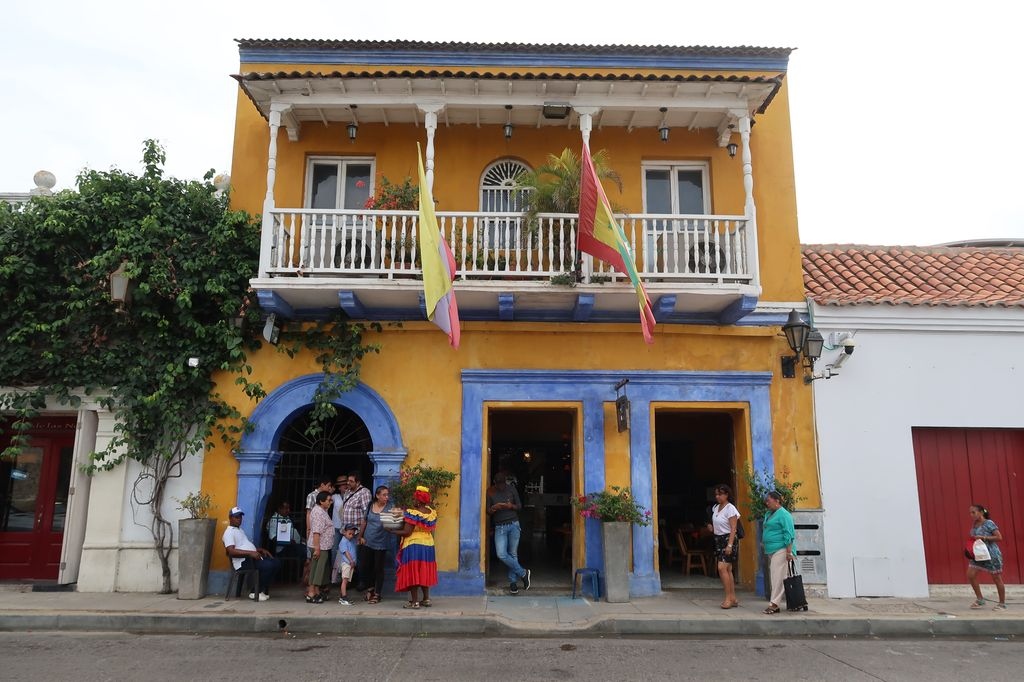
\includegraphics{images/20180917_rue.JPG}
\caption{On trouve de belles couleurs dans les rues de Carthagène.}
\end{figure}

La réputation de Carthagène n'est plus à faire : haut lieu de tourisme,
la vieille ville entourée de remparts est classée à l'UNESCO et les
buildings de Bocagrande accueillent à bras ouverts les touristes de tout
le continent américain désireux de se défaire de quelques dollars.
Située sur la côte nord de la Colombie, donnant sur la mer des Caraïbes
et offrant un climat tropical, cette petite ville a donc tout pour
plaire. Mais ça, c'est sur le papier !

En pratique, notre séjour n'a pas pris le tour paradisiaque qu'on
espérait (même si ça restait agréable). La densité de vendeurs de rues
est telle qu'on se fait accoster des dizaines et des dizaines de fois
par jour. Pour une excursion touristique, pour un massage, pour un
restaurant, pour une bière... ça n'en finit jamais. Au point que cela
devient parfois drôle (quand on énumère la liste des plats de concert
avec le serveur d'un resto de notre rue) ou glauque (quand la masseuse
qui passe à côté de nous sur la plage insiste lourdement pour nous
enduire d'huile). D'autant plus que notre arrivée à Carthagène a été
particulièrement ratée : arnaque au taux de change (+ 50\%, tout de
même) et chauffard de taxi qui percute une voiture à contresens à force
de vouloir doubler (avec pour seul réaction le mot \emph{puta}, l'œil
rivé au rétro pour voir si nous étions poursuivi par la voiture
emboutie).

Ajoutez à ça les 28 degrés à cent pour cent d'humidité (auquel le Pérou
ne nous avait pas préparé) qui nous font mal dormir, il nous a fallu
quelques jours de \emph{farniente} pour nous en remettre et avant
d'apprécier le paysage.

Heureusement, la vieille ville de Carthagène vaut le détour. Construite
par les Espagnols (encore eux !), son port a servi à transborder les
richesses incroyables tirées de la conquête du Pérou et de la Colombie.
Un \emph{free walking tour} (encore un !) nous rend familier de
l'histoire de la colonie, de la traite des esclaves ou encore des
différents assauts donnés à la ville par les britanniques, les français
ou les américains. Notre expertise des \emph{free walking tour},
accumulée de Santiago à Lima, nous permet à cette occasion de remporter
plusieurs quizz et même le maillot de foot de l'équipe nationale lors de
l'épreuve finale (qui s'avérera en fait être un porte-clé).

\begin{figure}
\centering
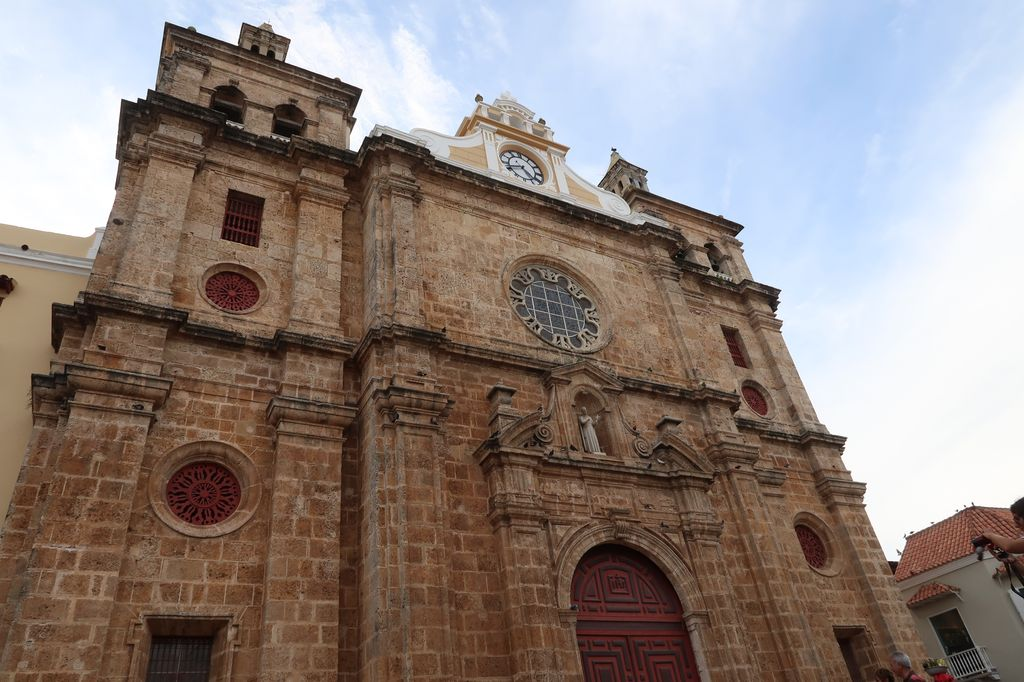
\includegraphics{images/20180917_sanpedro.JPG}
\caption{L'église de San Pedro Claver.}
\end{figure}

Nous faisons également la rencontre d'Ernesto, qui nous conduira à
différents endroits autour de la ville dans son taxi (notamment le fort
de San Felipe et le monastère de la Popa) et nous fera goûter quelques
spécialités locales cuites dans la rue : \emph{arepa con huevo} (dont il
faut toujours manger deux unités tellement c'est bon) et
\emph{carimañola} (à base de yucca). Miam.

\begin{figure}
\centering
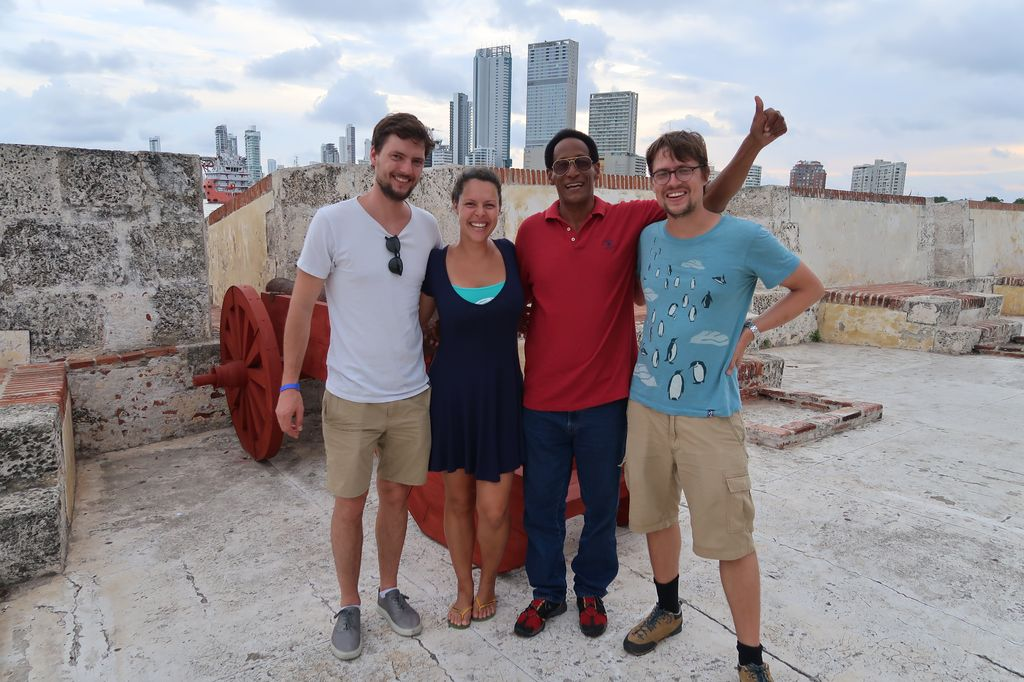
\includegraphics{images/20180917_ernesto.JPG}
\caption{Ernesto, toujours prêt à dire "chebere" (super) !}
\end{figure}

Enfin, il y a les excursions. Comme nous ne faisons rien sans consulter
internet, nous décidons de ne pas aller à Playa Blanca (trop
touristique) et optons pour \emph{el Encanto}, une plage privée dans les
\emph{islas del Rosario}. C'est pas si mal, mais à force de voir des
plages de rêve avec peu de touristes en Polynésie, on apprécie moins ce
genre d'endroit. La surprise agréable ce sera finalement l'excursion au
"volcan" Totumo pour un bain de boue. Le terme de volcan est sans aucun
doute usurpé, mais la sensation de flottaison dans un bon bain de boue
est étonnante. Et le repas inclus dans l'excursion nous réconcilie avec
son caractère touristique.

\begin{figure}
\centering
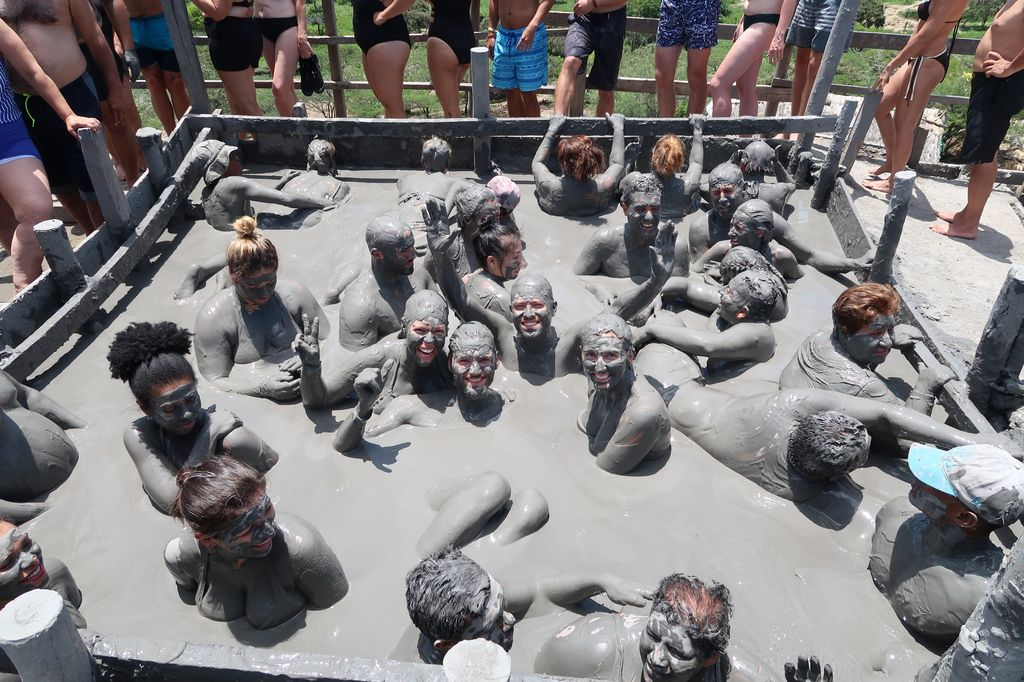
\includegraphics{images/20180917_totumo.JPG}
\caption{Le bassin de boue n'est pas très grand, tout le monde doit
attendre son tour.}
\end{figure}

Et dire qu'on était venu à Carthagène pour donner l'occasion à Raphaël
de surfer... Les vagues ne sont pas au rendez-vous même lorsqu'on est à
la plage à six heures du matin. Tant pis, ce sera donc notre bain de mer
le plus matinal de tout le séjour :D.

\begin{figure}
\centering
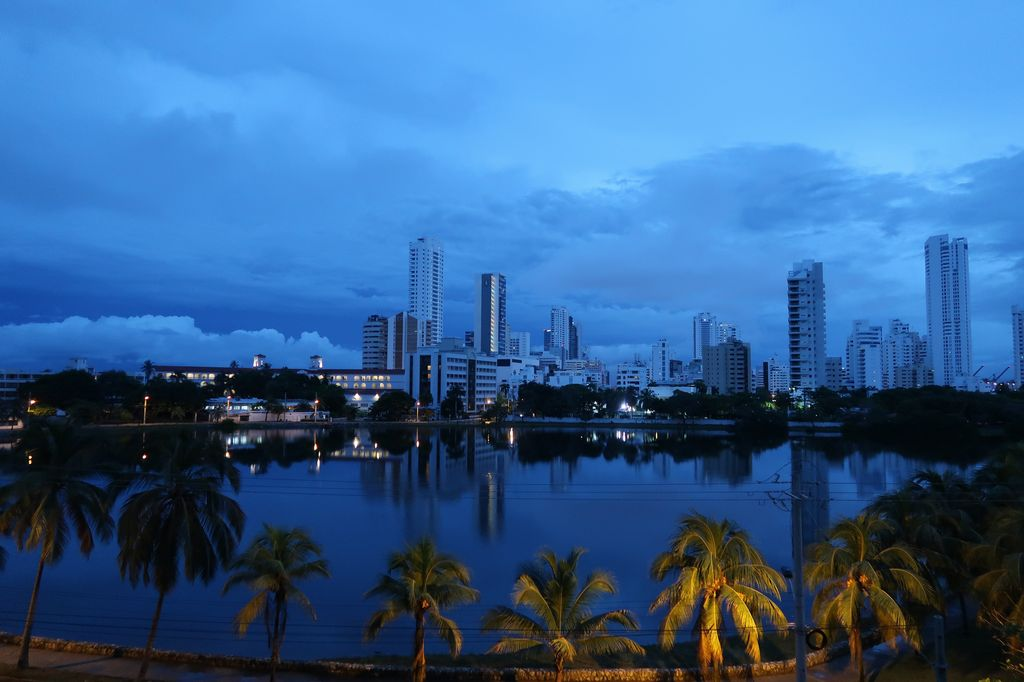
\includegraphics{images/20180917_laguito.JPG}
\caption{L'avantage de se lever à 5h du matin, c'est qu'on peut profiter
de l'heure bleue pour faire ce genre de photo.}
\end{figure}

Nous sommes tristes de quitter Lisa et Raphaël le dernier jour. Pour
eux, c'est le retour (surtout pour Lisa, après 7 mois passés au Brésil,
chapeau !) alors que nous avons la chance de continuer le voyage vers
Mexico. Et finalement, le vent a tourné (ou plutôt les vagues), et c'est
grâce à un vol un peu plus tardif que le nôtre que Raph a pu prendre
quelques vagues avant de partir à son tour !

\emph{Florian}
